\documentclass{bioinfo}
\copyrightyear{2019} \pubyear{2019}

\access{Advance Access Publication Date: Day Month Year}
\appnotes{Applications Note}

\begin{document}
\firstpage{1}

\subtitle{Genetic and population analysis}

\title[Unified power analysis and forensics of association studies]{U-PASS: unified power analysis and forensics for qualitative traits in genetic association studies}
\author[Gao \textit{et~al}.]{Zheng Gao\,$^{\text{\sfb 1,}*}$, Jonathan Terhorst\,$^{\text{\sfb 1}}$, Cristopher Van Hout\,$^{\text{\sfb 2}}$, and Stilian Stoev\,$^{\text{\sfb 1}}$}
\address{$^{\text{\sf 1}}$Department of Statistics, University of Michigan, Ann Arbor, MI 48109, USA and \\
$^{\text{\sf 2}}$Regeneron Genetics Center, Tarrytown, NY 10591
USA.}

\corresp{$^\ast$To whom correspondence should be addressed.}

\history{Received on XXXXX; revised on XXXXX; accepted on XXXXX}

\editor{Associate Editor: XXXXXXX}

\abstract{
\textbf{Summary:} 
Despite the availability of existing calculators for statistical power analysis in genetic association studies, there has not been a model-invariant and test-independent tool that allows for both planning of prospective studies and systematic review of reported findings.
In this work, we develop a web-based application U-PASS (Unified Power analysis of ASsociation Studies), implementing a unified framework for the analysis of common association tests for binary qualitative traits.
The application quantifies the shared asymptotic power limits of the common association tests, and visualizes the fundamental statistical trade-off between risk allele frequency (RAF) and odds ratio (OR). 
The application also addresses the applicability of asymptotics-based power calculations in finite samples, and provides guidelines for single-SNP-based association tests. 
In addition to designing prospective studies, U-PASS enables researchers to retrospectively assess the statistical validity of previously reported associations.\\
\textbf{Availability and implementation:} U-PASS is an open-source R Shiny application. A live instance is hosted at {https://power.stat.lsa.umich.edu}. 
Source is available on {https://github.com/Pill-GZ/U-PASS}.\\ %License information will be available in the repo?
\textbf{Contact:} \href{gaozheng@umich.edu}{gaozheng@umich.edu}\\
\textbf{Supplementary information:} Supplementary data are available at \textit{Bioinformatics}
online.}
\maketitle

\section{Introduction}
\label{sec:intro}
The probability of detecting a true association between genetic and phenotype variations, known as statistical power, is influenced by a number of factors such as sample sizes, the statistical test used, the frequency of the risk variant, and magnitude of the effect on the trait. 
Power analysis, which determines the suitable factor combinations in order to achieve sufficient statistical power, plays an important role in determining study designs \citep{Skol06, Goodwin16}, and in interpreting published findings \citep{Ioannidis05}.

There has been a number of widely used calculators for genome-wide association studies (GWAS). 
\cite{Sham98} studied power analysis of likelihood ratio tests for associations between marker SNPs and quantitative or qualitative traits; the results were implemented in GPC \citep{Purcell03}.
\cite{Skol06} studied the performance of two-sample t-tests, and extended the analysis to two-stage designs; the results were implemented in the CaTS caclulator, and later, in the GAS calculator for one-stage designs \citep{Johnson17}.
Independently, \citet{Menashe08} implemented the calculations for one-stage designs in the PGA calculator.
Recent works have also studied power of a number of SNP-set based tests targeting rare variants \citep{Wang14, Derkach17}.
See \citet{Sham14} for a review.

Despite these efforts, some difficulties remain in practice:

%\vspace{-5pt}
% \begin{enumerate}
    %\noindent
    {\it 1. Lack of universality.} 
    Existing power analyses are tied to the underlying models and the statistical procedures used; power calculations for a certain model-method combination may not be valid if either the model or the method changes.
    % In principle, power calculations based on likelihood ratio tests or t-tests cease to hold for studies running logistic regressions or chi-squared tests.
    Users are burdened with matching the appropriate tool to the specific type of analysis they wish to perform.
    This is complicated by the fact that the precise test and model assumptions are rarely made explicit in the existing calculators.
    %Users have to match their tests used with that assumed by the power calculators, although these assumptions are rarely made explicit. 
    
    %\noindent
    {\it 2. Mismatching definitions of key quantities.}
    %A typical example is risk allele frequency (RAF), for which we identify at least three operational definitions (see Sec 2). 
    While GWAS catalogs, e.g., NHGRI-EBI \citep{MacArthur16}, require studies to report risk allele frequency (RAF) \emph{in the control group}, all of the aforementioned power calculators assume the RAF input to be the frequency \emph{in the general population}. 
    These quantities are not necessarily equal, and using one in place of the other may grossly distort power estimates.
    
    %\noindent
    {\it 3. (In)accuracies in finite samples.} While existing tools rely on large-sample approximations in their power calculations, these approximations are not reliable in finite samples when genetic variants are rare. Existing calculators are silent about the applicability of asymptotics-based approximations, and how they should be corrected.
% \end{enumerate}

As a result, it is not only challenging to use the existing power calculation tools for planning genetic association studies correctly, but also difficult to systematically review the statistical validity of findings reported in the literature, since different models and tests must be handled differently, and with care.

In an effort to address these difficulties and deficiencies, we propose a unified framework for power analysis of single variant association studies.
By abstracting away the assumptions of disease models and testing procedures which may vary from study to study, we reduce the problem to the essential quantities that are invariant to nuisance parameters. 
These ideas are implemented in the software U-PASS, enabling model-invariant, test-independent power analysis, as well as systematic reviews of the statistical validity of reported findings.

We briefly summarize the important features and uses of the software below.
Mathematical details and results from numerical experiments are collected in the Supplement.



\vspace*{-16pt}
\section{Methods and features}
\label{sec:results}



%\vspace{-5pt}
\subsection{The canonical and disease model parametrizations}

We provide two methods of specifying the alternative hypothesis in power analysis.
In addition to the familiar option of specification through disease models, we provide users with the option to perform power analysis via the canonical parameters, whose estimates are curated and readily available in the NHGRI-EBI GWAS Catalog:
\begin{itemize}
    \item Conditional distribution of risk allele variant among controls, i.e., risk allele frequency (RAF) in the Control group, denoted as $f$.
    \item Odds ratio (OR) of allele variants, denoted as $\text{R}$.
\end{itemize}
The canonical parameters ($f$ and $R$) are common to models of qualitative traits and invariant to model choices. 
This disease model-invariance allows users to perform power analysis valid for studies employing different models.
We also elucidate on the link between the two approaches, and provide a ``disease model converter'' in the application, performing explicit conversions from the disease models to the canonical parametrizations.

% From a statistical perspective, the disease model serves no role except to specify the distribution of the counts under the alternative.
% Here, statistical power is calculated directly based the quartet $(n_1, n_2, f, R)$, allowing us to perform power analysis valid for studies employing different models.

% We make the important distinction between RAF in the Control group ($f$), versus RAF among all subjects in the study, and RAF in the general population.
% Throughout this work and the software, RAF refers to the risk allele frequency in the Control group, consistent with the reporting standard of the NHGRI-EBI GWAS Catalog.

\vspace{-5pt}
\subsection{A test-independent power analysis}

While power calculations are necessarily tied to the statistical tests used, for many common association tests, statistical powers are asymptotically equivalent.
% For example, it is known that for tests of associations in contingency tables, the likelihood ratio (LR) test and Pearson's chi-square test enjoy the same power asymptotically.
% We further show that tests including, e.g., Welch's t-test (though not the student t-test) and LR tests for logistic regressions, also have asymptotically the same power, as long as the canonical parameters assume the same values. 
We show in the Supplement that the likelihood ratio test, chi-square test, Welch's t-test, and LR test for logistic regressions have asymptotically the same power, as long as the canonical parameters assume the same values. 
Our model-invariant, test-independent analysis allows us to calculate power in a unified fashion. 
The formulas used for power calculations in terms of the canonical parameters are detailed in Section 1 of the Supplementary material.

%In the software, users need only prescribe the sample sizes. 
Our software only requires users to specify the number of cases and controls.
The common power limits are calculated as a function of RAF and OR, and visualized as a heatmap in the OR-RAF diagram.
%; see Figure \ref{fig:02} for a preview of the software graphical user interface.

% \begin{figure}[!tpb]%figure1
% 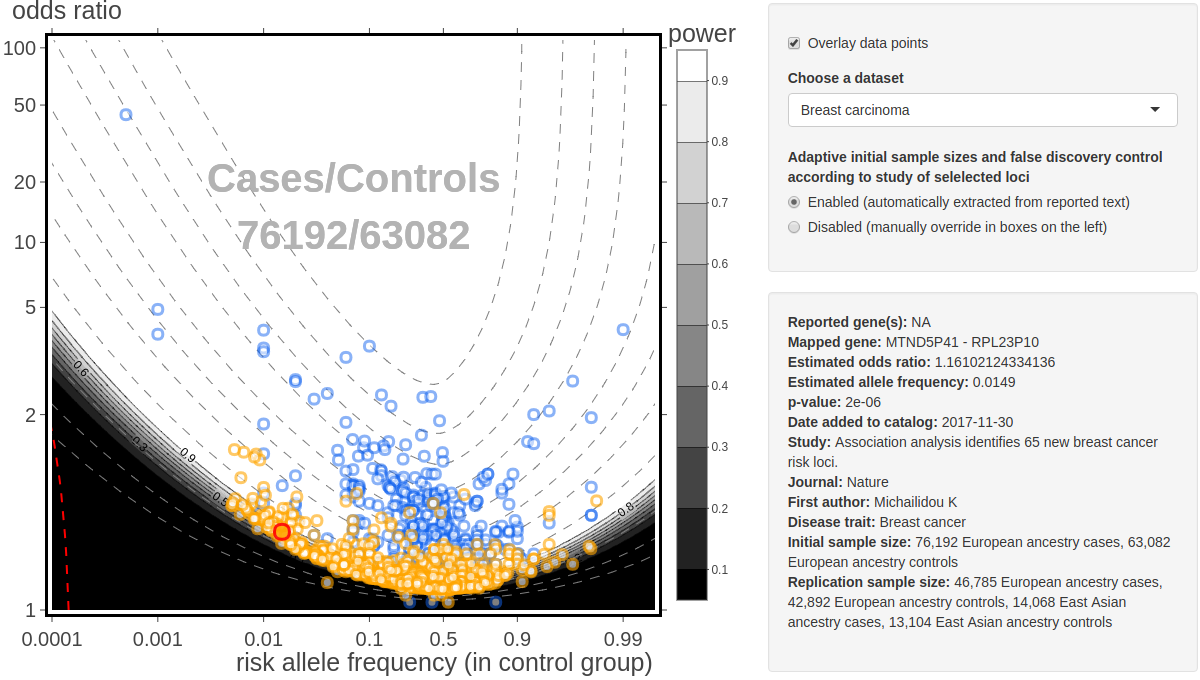
\includegraphics[width=0.48\textwidth]{Screenshot_GWAS_calculator6.eps}
% \vspace{-20pt}
% \caption{Snapshot of the application's user interface, displaying reported associations from breast cancer studies in the NHGRI-EBI GWAS Catalog (circles).
% % the reported odds ratios and risk allele frequencies in the control groups. 
% The findings are overlaid on the OR-RAF power diagram of association tests (greyscale heatmap).
% The initial sample sizes are dynamically adjusted, and automatically determined from texts of the article reporting the user selected loci (red circle). 
% Information of the selected loci and the articles are also dynamically displayed; findings reported in the same article are highlighted (orange circles).
% We provide finite sample corrections by marking the rare variant region(s) where asymptotic approximations do not apply (red dashed lines, lower-left).
% The majority of the published findings we surveyed exhibited a striking level of concordance with our theoretical predictions, with most associations congregating just inside the detectable region.
% }\label{fig:02}
% \vspace{-12pt}
% \end{figure}

\vspace{-5pt}
\subsection{Review and forensics of reported findings}

This unified treatment allows us to examine results from different studies in the same diagram, even when they do not employ the same model or statistical test.
This enables systematic reviews of reported findings for their statistical validity. 
In particular, a reported association predicted to have low power given the study's sample size -- lying in the dark regions of the OR-RAF diagram -- while not impossible, invites further scrutiny.%\footnote{It should be noted that a reported association predicted to have high power is not automatically accurate, as winner's curse induced by multiple testing may inflate the OR and RAF estimates \citep{Xiao09}.}

Studies where reported associations show misalignment with the predicted powered curves may be further investigated for potential problems.
% For example, the results of \citet{Dominguez-Cruz18} appear grossly misaligned when visualized using our method.
We reached out to one study where gross misalignment was identified \citep{Dominguez-Cruz18}. 
% The authors of the study confirmed with us that the RAF reported in the Catalog were based on all subjects in the study, as opposed to only the control group.
The authors of the study confirmed that this was the result of a problem in the data curation process of the GWAS Catalog (Dominguez-Cruz, personal communication).

The software provides options for users to load and overlay findings reported in the NHGRI-EBI GWAS Catalog, or upload data from other sources compliant with the Catalog's data format.

% In particular, for large samples, tests for zero slopes in logistic regressions should report approximately the same set of loci as Welch's t-tests for equal proportions on the same dataset, after the same family-wise error rate adjustments.
% The estimated odds ratios (in the case of logistic regression, estimate slopes exponentiated) and RAF's, when charted on the OR-RAF diagram, should also follow the same power limits.


\vspace{-5pt}
\subsection{Rare variants and finite sample corrections}

We address the quality of asymptotic approximations in our power analysis, as well as the applicability of single variant tests when rare genetic variants are present.
Specifically, we provide a lower bound on the variant counts needed to calibrate Fisher's exact test. 
If variant counts fall below the threshold, exact tests, and by extension, single-SNP-based association tests, cannot be correctly calibrated to have the desired type I error rate  without sacrificing all statistical power.
In such cases, the asymptotic approximations do not apply.
We mark this low-count, low-power region on the OR-RAF diagram.
See Supplement Sec. 2 for further details.

The software also provides options for users to specify the rare variant as 1) having less than a specified count, or 2) occurring in less than a percentage of all subjects in the study, as is customary in the literature.






\vspace*{-16pt}
\section{Implementation}
\label{sec:implementaion}

U-PASS is implemented as an interactive web-based R Shiny application, hosted at {https://power.stat.lsa.umich.edu}, open to the public. 
%It has been designed to be user-friendly and self-contained.
%The software complies with the NHGRI-EBI GWAS Catalog data format.
Source code is freely available at {https://github.com/Pill-GZ/U-PASS}.


% \vspace*{-10pt}
% \section*{Acknowledgements}
% 
% We thank so and so for their invaluable comments and suggestions on the early versions of the software and this paper.

\vspace*{-16pt}
\section*{Funding}

This work is partially supported by NSF Grant DMS-1830293, ATD.
\vspace*{-16pt}

%\bibliographystyle{natbib}
%\bibliographystyle{achemnat}
%\bibliographystyle{plainnat}
%\bibliographystyle{abbrv}
%\bibliographystyle{bioinformatics}
%
%\bibliographystyle{plain}
%
%\bibliography{Document}


\begin{thebibliography}{}

\bibitem[Derkach {\it et~al}., 2017]{Derkach17}
Derkach, A., Zhang, H., \& Chatterjee, N. (2017). 
Power Analysis for Genetic Association Test (PAGEANT) provides insights to challenges for rare variant association studies. 
{\it Bioinformatics}, {\bf 34}, 1506-1513.

% \bibitem[Gonz\'{a}lez {\it et~al}., 2008]{Gonzalez08}
% Gonz\'{a}lez, J. R., Carrasco, J. L., Dudbridge, F., Armengol, L., Estivill, X., \& Moreno, V. (2008). 
% Maximizing association statistics over genetic models. 
% {\it Genetic Epidemiology}, {\bf 32(3)}, 246-254.

\bibitem[Dominguez-Cruz {\it et~al}., 2018]{Dominguez-Cruz18}
Dom\'inguez-Cruz, M. G., de Lourdes Mu\~noz, M., Totomoch-Serra, A., Garc\'ia-Escalante, M. G., Burgue\~no, J., Valadez-Gonz\'alez, N., ... \& D\'iaz-Badillo, \'A. (2018). 
Pilot genome-wide association study identifying novel risk loci for type 2 diabetes in a Maya population. 
{\it Gene}, {\bf 677}, 324-331.

\bibitem[Goodwin {\it et~al}., 2016]{Goodwin16}
Goodwin, S., McPherson, J. D., \& McCombie, W. R. (2016). 
Coming of age: ten years of next-generation sequencing technologies. 
{\it Nat. Reviews Genetics}, {\bf 17}, 333.

\bibitem[Ioannidis, 2005]{Ioannidis05}
Ioannidis, J. P. (2005).
Why most published research findings are false. 
{\it PLoS medicine}, {\bf 2}, e124.

\bibitem[Johnson {\it et~al}., 2017]{Johnson17}
Johnson, J. L., \& Abecasis, G. R. (2017). 
GAS Power Calculator: web-based power calculator for genetic association studies. 
{\it bioRxiv}, 164343.

% \bibitem[Li {\it et~al}., 2008]{Li08}
% Li, Q., Zheng, G., Li, Z., \& Yu, K. (2008). 
% Efficient approximation of P‐value of the maximum of correlated tests, with applications to genome‐wide association studies. 
% {\it Annals of human genetics}, {\bf 72(3)}, 397-406.

\bibitem[MacArthur {\it et~al}., 2016]{MacArthur16}
MacArthur, J., Bowler, E., Cerezo, M., Gil, L., Hall, P., Hastings, E., ... \& Pendlington, Z. M. (2016). 
The new NHGRI-EBI Catalog of published genome-wide association studies (GWAS Catalog). 
{\it Nucleic acids research}, {\bf 45}, D896-D901.

\bibitem[Menashe {\it et~al}., 2008]{Menashe08}
Menashe, I., Rosenberg, P. S., \& Chen, B. E. (2008). 
PGA: power calculator for case-control genetic association analyses. 
{\it BMC genetics}, {\bf 9}, 36.

\bibitem[Purcell {\it et~al}., 2003]{Purcell03}
Purcell, S., Cherny, S. S., \& Sham, P. C. (2003). 
Genetic Power Calculator: design of linkage and association genetic mapping studies of complex traits. 
{\it Bioinformatics}, {\bf 19}, 149-150.

\bibitem[Sham, 1998]{Sham98}
Sham, P. C. (1998). {\it Statistics in human genetics}. Wiley.

\bibitem[Sham  \& Purcell, 2014]{Sham14}
Sham, P. C., \& Purcell, S. M. (2014).
Statistical power and significance testing in large-scale genetic studies. 
{\it Nature Reviews Genetics}, {\bf 15}, 335.

\bibitem[Skol {\it et~al}., 2006]{Skol06}
Skol, A. D., Scott, L. J., Abecasis, G. R., \& Boehnke, M. (2006). 
Joint analysis is more efficient than replication-based analysis for two-stage genome-wide association studies. 
{\it Nature genetics}, {\bf 38}, 209.

\bibitem[Wang {\it et~al}., 2014]{Wang14}
Wang, G. T., Li, B., Lyn Santos-Cortez, R. P., Peng, B., \& Leal, S. M. (2014). 
Power analysis and sample size estimation for sequence-based association studies. 
{\it Bioinformatics}, {\bf 30}, 2377-2378.

% \bibitem[Xiao \& Boehnke, 2009]{Xiao09}
% Xiao, R., \& Boehnke, M. (2009). 
% Quantifying and correcting for the winner's curse in genetic association studies. 
% {\it Genetic Epidemiology}, {\bf 33(5)}, 453-462.

% \bibitem[Lee {\it et~al}., 2014]{Lee2014}
% Lee, S., Abecasis, G. R., Boehnke, M., \& Lin, X. (2014). Rare-variant association analysis: study designs and statistical tests. 
% {\it The American Journal of Human Genetics}, {\bf 95(1)}, 5-23.

\end{thebibliography}
\end{document}

